% 图 B.2 方形元电流环（逆时针电流）与 x、y 轴
\documentclass[tikz,border=5pt]{standalone}
\usetikzlibrary{arrows.meta}
\usepackage{amsmath}
\usepackage{bm}
\usepackage{fontspec}
\setmainfont{Times New Roman}
\begin{document}
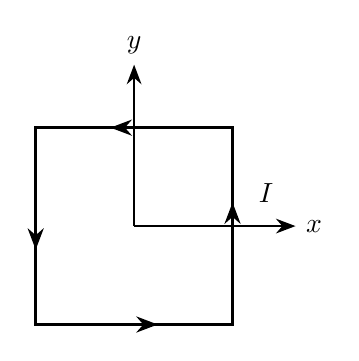
\begin{tikzpicture}[line width=0.9pt,>=Stealth]
% square loop
\draw (-1.25,-1.25) rectangle (1.25,1.25);
% current direction (anticlockwise)
\draw[->,line width=1.05pt] (1.25,-0.30) -- (1.25,0.30);
\node[right] at (1.45,0.42) {$I$};
\draw[->,line width=1.05pt] (0.30,1.25) -- (-0.30,1.25);
\draw[->,line width=1.05pt] (-1.25,0.30) -- (-1.25,-0.30);
\draw[->,line width=1.05pt] (-0.30,-1.25) -- (0.30,-1.25);
% axes
\draw[->] (0,0) -- (2.05,0) node[right] {$x$};
\draw[->] (0,0) -- (0,2.05) node[above] {$y$};
\end{tikzpicture}
\end{document}
